\documentclass[12pt,fleqn]{article}\usepackage{../../common}
\begin{document}
Dalga Denklemi Hesabı

Önce ip üzerinde titreşimlerin hareketi sonucu olan dalga denklemini
türetelim. Bu türetimin bir şeklini [1]'de görmüştük, şimdi [2,3,4] bazlı olarak
tekrar görelim.

Bir ipte dalga onun salınımı ile oluşacak, ve bu salınım sırasında bir anda, tek
bir fotoğraf karesinde görüntü alt soldaki gibi olabilir, 

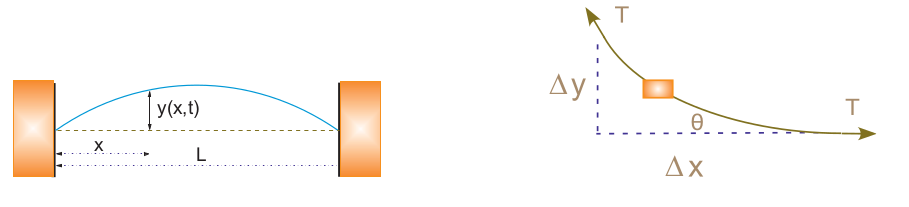
\includegraphics[width=30em]{compscieng_app17wave_01.png}

İp iki tarafından hareket etmeyen yerlere bağlanmış (duvar mesela) uzunluk $L$,
ip materyelinin yoğunluğu $\rho$, ki bu tüm ipin kütlesi bölü uzunluğu olarak ta
görülebilir, bu örnekte sabit, ipin gerginliği kuvvet olarak $T$, bu da sabit,
ve yerçekimi kuvvetine göre çok daha fazla böylece yerçekim ivmelenmesi $g$'yi
yok sayabiliyoruz. Sürtünme yok. Tek boyutta bakıyoruz, $y(x,t)$ ipin bir $x$
noktasındaki dikey yer değişimini gösteriyor.

Denklemi ortaya çıkartmak için aslında Newton'un $F=ma$'sından daha fazlasına
ihtiyacımız yok. Üst sağdaki resimde gösterildiği gibi tek bir sonsuç ufak
bölgeye odaklanırsak, ya da alt resimde olduğu gibi,

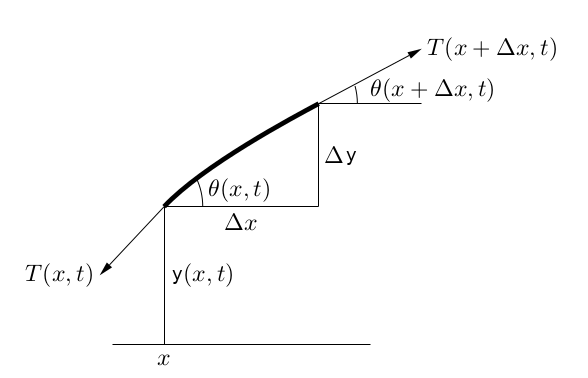
\includegraphics[width=20em]{compscieng_app17wave_02.png}

$F$ için gereken net kuvveti ipin iki yanyana noktası arasındaki gerginliğin
dikey bileşenlerinin farkı olarak görebiliriz, yani $T(x+\Delta x,t)$ ve
$T(x,t)$ kuvvetlerinin dikey bileşen farkı. İki noktadaki acılar da
$\theta(x,t)$ ile gösteriliyor, $x+\Delta x$'teki acı $\theta(x+\Delta x)$. Bu
dikey bileşenlerin farkını, ya da tüm $y$ kuvvetlerinin toplanını o zaman 

$$
\sum F_y = T(x+\Delta x,t) \sin\theta(x+\Delta x,t) - T(x,t) \sin\theta(x,t)
$$

ile hesaplayabiliriz. Modeldeki faraziyeler isiginda biliyoruz ki $y/L$ cok
kucuk, o zaman $\theta$ cok kucuk. Demek ki sinus ifadelerini
basitlestirebiliriz, [5]'ten biliyoruz ki

$$
\sin\theta \approx \tan\theta = \partial y / \partial x
$$

Demek ki

$$
\sum F_y =
T \frac{\partial y}{\partial x} \bigg\vert_{x+\Delta x} -
T \frac{\partial y}{\partial x} \bigg\vert_{x}
$$

Son geldiğimiz noktada birinci türevler üzerinden bir $x$ farklılığı görüyoruz,
bu bize bir türev işlemini daha hatırlatıyor, eğer $\Delta x$ ile bölünme de
olsaydı, o zaman ikinci türev elde ettik diyebilirdik,

$$
\frac{
T \frac{\partial y}{\partial x} \bigg\vert_{x+\Delta x} -
T \frac{\partial y}{\partial x} \bigg\vert_{x}
}{\Delta x} \approx T \frac{\partial^2 y}{\partial x^2}
$$

Fakat önemli değil, biraz masajlama yaparsak, 

$$
T \frac{\partial y}{\partial x} \bigg\vert_{x+\Delta x} -
T \frac{\partial y}{\partial x} \bigg\vert_{x} \approx
T \frac{\partial^2 y}{\partial x^2} \Delta x 
$$

İstenilen sonucu elde ederiz, 

$$
\sum F_y \approx T \frac{\partial^2 y}{\partial x^2} \Delta x
$$

Diğer taraftan $F=ma$ eşitliğinin sağ tarafına bakarsak, baktığımız ufak bölge
için kütle $\rho\Delta x$, yatay ivmelenme ise $y$ yer değişiminin zamana göre
ikinci kısmi türevi,

$$
\sum F_y = \rho \Delta x \frac{\partial^2 y}{\partial t^2}
$$

Bu son iki denklemi birbirine eşitlersek, $\Delta x$'ler iptal olur, 

$$
T \frac{\partial^2 y}{\partial x^2}  =
\rho \frac{\partial^2 y}{\partial t^2}
$$

Sabitleri sağ tarafa taşırsak, ve $c = \sqrt{T / \rho}$ tanımı üzerinden,

$$
\frac{\partial^2 y}{\partial x^2}  =
\frac{1}{c^2}\frac{\partial^2 y}{\partial t^2}
$$

Dalga denklemini elde etmiş olduk.

Denkleme yakından bakarsak onun bir kısmı türevsel denklem (PDE) olduğunu
görürüz. İki tane bağımsız değişken temel alınıyor, $x,t$. Ayrıca denklem
2. derece, çünkü ikinci türevi içeriyor. Bu bilgiler denklemi çözmek için
önemli.

Çözümde bir başlangıç şartı gerekli çünkü diferansiyel denklemleri ``entegre
ederken'' daha doğrusu ileri doğru geçen zamanda hesaplarken bir başlangıç
noktası gerekiyor, bunun için bir teli kaldırıp (geçici bir süre üçgen haline
getirip) oradan bıraktığımızı düşünebiliriz, ki bu üçgen şekli alttaki gibi
modellenebilir,

$$
y(x,t=0)=\begin{cases}
1.25 x/L , &x\leq 0.8 L ,\\
(5-5x/L), &x> 0.8 L,
\end{cases} 
$$

İkinci bir başlangıç şartı daha lazım, 2. derece başlangıç şartı bu. Teli, ipi
gerip üçgen yaptım ama sonra durup tekrar bıraktım, bu da bir başlangıç şartı,
durağan durumdan başlama şartı.

$$
\frac{\partial y} {\partial t}(x,t=0) =0
$$

Cozume bu sartlarla baslayabilirdik ama bastaki problem tanimini hatirlarsak ek
bazi sartlar daha koymustuk, bu sartlar, kisitlamalar her an icin gecerli,
ipler iki ucundan (hareket etmeyen) duvarlara bagli.

$$
y(0,t) \equiv 0, \quad y(L,t) \equiv 0
$$

[analitik çözüm atlandi]

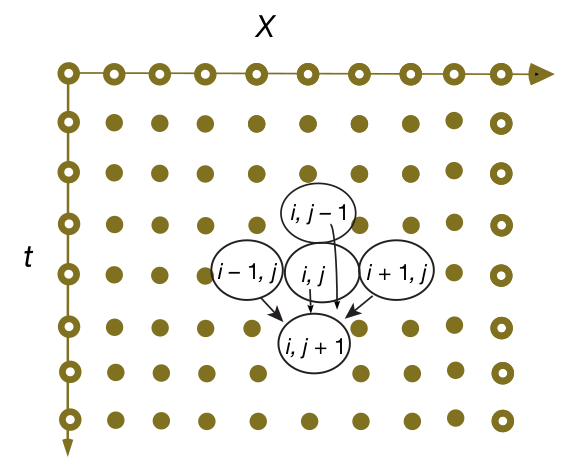
\includegraphics[width=20em]{compscieng_app17wave_03.png}

$$
\frac{\partial^2 y }{\partial t^2} \simeq
\frac{y_{i,j+1}+y_{i,j-1}-2 y_{i,j}}{(\Delta t)^2}, \quad
\frac{\partial^2 y}{\partial x^2} \simeq
\frac{y_{i+1,j}+y_{i-1,j}-2 y_{i,j}} {(\Delta x)^2}.
$$

$$
\frac{y_{i,j+1}+y_{i,j-1}-2 y_{i,j}} {c^2 (\Delta t)^2}  =
\frac{y_{i+1,j}+y_{i-1,j}-2 y_{i,j}} {(\Delta x)^2}
$$












[devam edecek]

Kaynaklar

[1] Bayramlı, {\em PDE, Dalga Denklemini Türetmek}

[2] Landau, {\em Landau Computational Physics Course, Video Lectures},
    \url{https://www.youtube.com/playlist?list=PLnWQ_pnPVzmJnp794rQXIcwJIjwy7Nb2U}

[3] Landau, {\em Computational Physics}

[4] Feldman, {\em Math 256, Differential Equations, Lecture Notes}
    \url{http://www.math.ubc.ca/~feldman/m256/}

[5] Bayramli, {\em Normal Diferansiyel Denklemler Ders Notlari, Ekler, Trigonometri}
    
\end{document}


